\documentclass[12pt]{report}
\usepackage[spanish]{babel}
\usepackage[utf8]{inputenc}
\usepackage{amsmath}
\usepackage{amssymb}
\usepackage{amsthm}
\usepackage{graphics}
\usepackage{subfigure}
\usepackage{lipsum}
\usepackage{array}
\usepackage{multicol}
\usepackage{enumerate}
\usepackage[framemethod=TikZ]{mdframed}
\usepackage[a4paper, margin = 1.5cm]{geometry}

%En esta parte se hacen redefiniciones de algunos comandos para que resulte agradable el verlos%

\renewcommand{\theenumii}{\roman{enumii}}

\def\proof{\paragraph{Demostración:\\}}
\def\endproof{\hfill$\blacksquare$}

\def\sol{\paragraph{Solución:\\}}
\def\endsol{\hfill$\square$}

%En esta parte se definen los comandos a usar dentro del documento para enlistar%

\newtheoremstyle{largebreak}
  {}% use the default space above
  {}% use the default space below
  {\normalfont}% body font
  {}% indent (0pt)
  {\bfseries}% header font
  {}% punctuation
  {\newline}% break after header
  {}% header spec

\theoremstyle{largebreak}

\newmdtheoremenv[
    leftmargin=0em,
    rightmargin=0em,
    innertopmargin=-2pt,
    innerbottommargin=8pt,
    hidealllines = true,
    roundcorner = 5pt,
    backgroundcolor = gray!60!red!30
]{exa}{Ejemplo}[section]

\newmdtheoremenv[
    leftmargin=0em,
    rightmargin=0em,
    innertopmargin=-2pt,
    innerbottommargin=8pt,
    hidealllines = true,
    roundcorner = 5pt,
    backgroundcolor = gray!50!blue!30
]{obs}{Observación}[section]

\newmdtheoremenv[
    leftmargin=0em,
    rightmargin=0em,
    innertopmargin=-2pt,
    innerbottommargin=8pt,
    rightline = false,
    leftline = false
]{theor}{Teorema}[section]

\newmdtheoremenv[
    leftmargin=0em,
    rightmargin=0em,
    innertopmargin=-2pt,
    innerbottommargin=8pt,
    rightline = false,
    leftline = false
]{propo}{Proposición}[section]

\newmdtheoremenv[
    leftmargin=0em,
    rightmargin=0em,
    innertopmargin=-2pt,
    innerbottommargin=8pt,
    rightline = false,
    leftline = false
]{cor}{Corolario}[section]

\newmdtheoremenv[
    leftmargin=0em,
    rightmargin=0em,
    innertopmargin=-2pt,
    innerbottommargin=8pt,
    rightline = false,
    leftline = false
]{lema}{Lema}[section]

\newmdtheoremenv[
    leftmargin=0em,
    rightmargin=0em,
    innertopmargin=-2pt,
    innerbottommargin=8pt,
    roundcorner=5pt,
    backgroundcolor = gray!30,
    hidealllines = true
]{mydef}{Definición}[section]

\newmdtheoremenv[
    leftmargin=0em,
    rightmargin=0em,
    innertopmargin=-2pt,
    innerbottommargin=8pt,
    roundcorner=5pt
]{excer}{Ejercicio}[section]

%En esta parte se colocan comandos que definen la forma en la que se van a escribir ciertas funciones%

\newcommand\abs[1]{\ensuremath{\left|#1\right|}}
\newcommand\divides{\ensuremath{\bigm|}}
\newcommand\cf[3]{\ensuremath{#1:#2\rightarrow#3}}
\newcommand\natint[1]{\ensuremath{\left[\!\left[ #1\right]\!\right]}}
\newcommand{\afa}{\:
    \begin{tikzpicture}
        \draw [line width = 0.17 mm, black] (0,0) -- (-0.115,0.29);
        \draw [line width = 0.17 mm, black] (0,0) -- (0.115,0.29);
        \draw [line width = 0.17 mm, black] (-0.12,0) arc (190:-10:0.12cm);
    \end{tikzpicture}
    \:
}
%Este símvolo es para casi todo salvo una cantidad finita

%recuerda usar \clearpage para hacer un salto de página

\newcounter{figcount}
\setcounter{figcount}{1}

\begin{document}
    \setlength{\parskip}{5pt} % Añade 5 puntos de espacio entre párrafos
    \setlength{\parindent}{12pt} % Pone la sangría como me gusta
    \title{Notas Taller Topología Algebraica}
    \author{Cristo Daniel Alvarado}
    \maketitle

    \tableofcontents %Con este comando se genera el índice general del libro%

    %\setcounter{chapter}{3} %En esta parte lo que se hace es cambiar la enumeración del capítulo%
    
    \chapter{El Teorema de Seifert Van Kampen. Aplicaciones}
    
    \section{Introducción}
    
    Hasta ahora, hemos determinado la estructura del grupo fumdamental de muy pocos espacios. Para aplicar el grupo fundamental en más variedad de problemas, es necesario obtener métodos para determinar la estructura de más espacios.

    Haremos una pequeña enunciación del problema a tratar: Suponga que queremos determinar el grupo fundamental de un espacio $X$ (espacio arco-conexo). Siendo
    \begin{equation*}
        X=U\cup V
    \end{equation*}
    con $U,V$ dos subespacios de $X$ que son arco-conexos. Eligiendo un punto base $x_0\in U\cap V$, uno espera que haya alguna relación entre los grupos
    \begin{equation*}
        \pi(U,x_0)\quad\textup{y}\quad\pi(V,x_0)
    \end{equation*}
    misma que nos permita decir algo sobre $\pi(X,x_0)$. Nuestro objetivo será intentar determinar y decir algo sobre $\pi(X,x_0)$ bajo estas condiciones.

    \section{Declaración y Prueba del Teorema}

    Primero, estableceremos el problema. Suponga que $U$ y $V$ son subconjuntos arco-conexos abiertos de $X$ tales que $X=U\cup V$, y que $U\cap V$ es arco-conexo no vacío. Eliga un punto base $x_0\in U\cap V$ para todos los grupos a considerar.

    \begin{theor}[\textbf{Teorema de Seifert Van Kampen}]
        Sea $H$ cualquier grupo y $\rho_1,\rho_2,\rho_3$ tres homomorfismos cualesquiera tales que el diagrama

        \begin{minipage}{\textwidth}
            \begin{center}
                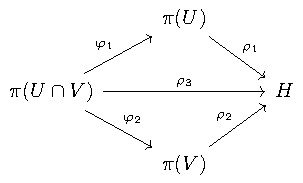
\includegraphics[scale=1.5]{images/fig_1.pdf}\\
                Figura \thefigcount. Diagrama conmutativo de los Grupos Fundamentales con $H$.
                \stepcounter{figcount}
            \end{center}
        \end{minipage}

        es conmutativo. Entonces, existe un único homomorfismo $\cf{\sigma}{\pi(X)}{H}$ tal que los siguientes tres diagramas son conmutativos:

        \begin{minipage}{\textwidth}
            \begin{center}
                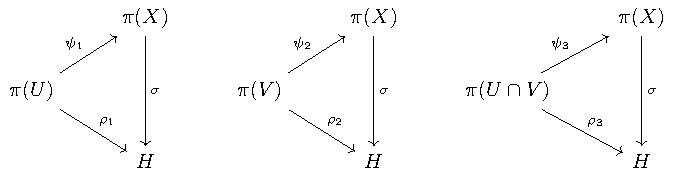
\includegraphics[scale=1.5]{images/fig_2.pdf}\\
                Figura \thefigcount. Diagramas conmutativo de $\pi(X)$ y $H$.
                \stepcounter{figcount}
            \end{center}
        \end{minipage}

        (donde los homomorfismos $\varphi_i$ y $\psi_i$ están inducidos por el mapeo inclusión, para $i=1,2,3$). Más aún, $\pi(X)$ está caracterizado hasta isomorfismos.
    \end{theor}

    Esta fue la primera versión del teorema que se probó (en su versión de dos espacios). No es nuestro objetivo actual el probar tal versión, sino una más general que involucre una cantidad arbitraria de componentes abiertas $U$ y $V$. Se verá de forma inmediata que con el siguiente teorema.

    Para ello, enunciaremos las condiciones que se requieren:

    \renewcommand{\theenumi}{\alph{enumi}}
    \begin{enumerate}
        \item $X$ es un espacio arco-conexo con $x_0\in X$.
        \item  $\left\{U_\lambda \right\}_{\lambda\in\Lambda}$ es una cubierta abierta de conjuntos arco-conexos de $X$ tales que $x_0\in U_\lambda$ para todo $\lambda\in\Lambda$.
        \item Para todo $\lambda_1,\lambda_2\in\Lambda$ existe $\lambda\in\Lambda$ tal que $U_{\lambda_1}\cap U_{\lambda_2}=U_\lambda$.
    \end{enumerate}

    la condicioń (c) también se enuncia diciendo que $\left\{U_\lambda \right\}_{\lambda\in\Lambda}$ es \textbf{cerrada bajo intersecciones finitas}.

    Consideraremos los grupos fundamnetales con punto base $x_0$.

    \begin{itemize}
        \item[(*)] Si $U_\lambda\subseteq U_\mu$, entonces la función
        \begin{equation*}
            \cf{\varphi_{ \lambda\mu}}{\pi(U_\lambda)}{U_\mu}
        \end{equation*}
        denota al homomorfismo inducido por el mapeo inclusión.
        \item[(**)] Similarmente, para todo índice $\lambda\in\Lambda$:
        \begin{equation*}
            \cf{\psi_\lambda}{\pi(U_\lambda)}{\pi(X)}
        \end{equation*}
        denota al homomorfismo inducido por el mapeo inclusión.
    \end{itemize}

    Note en particular, que si $U_\lambda\subseteq U_\mu$, entonces el diagrama

    \begin{minipage}{\textwidth}
        \begin{center}
            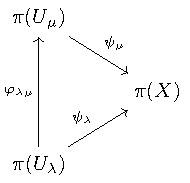
\includegraphics[scale=1.5]{images/fig_3.pdf}\\
            Figura \thefigcount. Diagramas conmutativo de $\pi(X)$, $\pi(U_\lambda)$ y $\pi(U_\mu)$.
            \stepcounter{figcount}
        \end{center}
    \end{minipage}

    es conmutativo. Ahora sí con el teorema general.

    \begin{theor}
        Bajo las hipótesis anteriores, el grupo $\pi(X)$ satisface la siguiente condición de \textit{mapeo universal}: Sea $H$ cualquier grupo, y para cada $\lambda\in\Lambda$ sea $\cf{\rho_\lambda}{\pi(U_\lambda)}{H}$ un homomorfismo, tales que la familia $\left\{\rho_\lambda \right\}_{\lambda\in\Lambda}$ satisface que el siguiente diagrama

        \begin{minipage}{\textwidth}
            \begin{center}
                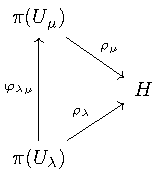
\includegraphics[scale=1.5]{images/fig_4.pdf}\\
                Figura \thefigcount. Diagramas conmutativo de $H$, $\pi(U_\lambda)$ y $\pi(U_\mu)$.
                \stepcounter{figcount}
            \end{center}
        \end{minipage}

        es conmutativo, para todo $\lambda,\mu\in\Lambda$ tales que $U_\lambda\subseteq U_\mu$. Entonces, existe un único homomorfismo $\cf{\sigma}{\pi(X)}{H}$ tal que para todo $\lambda\in\Lambda$ el siguiente diagrama

        \begin{minipage}{\textwidth}
            \begin{center}
                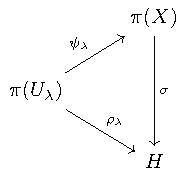
\includegraphics[scale=1.5]{images/fig_5.pdf}\\
                Figura \thefigcount. Diagramas conmutativo de $H$, $\pi(X)$ y $\pi(U_\lambda)$.
                \stepcounter{figcount}
            \end{center}
        \end{minipage}

        es conmutativo. Más aún, esta condición de mapeo universal caracteriza $\pi(X)$ hasta isomorfismos.
    \end{theor}

    Antes de hacer la prueba de este teorema, haremos la prueba de un lema que nos servirá para el teorema.

    \begin{lema}
        El grupo $\pi(X)$ es generado por la unión de las imágenes $\psi_\lambda\left(\pi(U_\lambda)\right)$, $\lambda\in\Lambda$.
    \end{lema}

    \begin{proof}
        %TODO
    \end{proof}


\end{document}